\definizione{
Data $ f: I\to \R $, $ f $\marginnote{1 dic 2021} derivabile in $ I\setminus \{x_0\} $, $ f $ continua in $ x_0 $, se \[
    \lim_{x\to x_0} f'(x) = \pm \infty
\]
allora $ x_0 $ è un \textit{flesso a tangente verticale}.

In $ x_0 $ la tangente al grafico è verticale}
\esempio{}{
    $ f(x)=\sqrt[3]{x} $, derivabile in $ \R\setminus\{0\} $ \[
        f'(x)_{x\neq 0}=\frac{1}{3\sqrt[3]{x}} \xrightarrow[x\to 0]{} +\infty \displaystyle
    \]
}

\definizione{
    Data $ f: I\to \R $, $ f $ derivabile in $ I\setminus \{x_0\} $, $ f $ continua in $ x_0 $, se \[
    \lim_{x\to x_0^{+}} f'(x) = + \infty\:\land\: \lim_{x\to x_0^{-}} f'(x) = - \infty
\]
oppure
\[
    \lim_{x\to x_0^{+}} f'(x) = - \infty\:\land\: \lim_{x\to x_0^{-}} f'(x) = + \infty
\]
allora $ x_0 $ è detto \textit{cuspide}.
}{}

% FOTO 2

\section{Teoremi per le funzioni derivabili}

\subsection{Teorema di Fermat}

\esempi{}{
    \begin{enumerate}
        \item La funzione 
        
        \begin{center}
            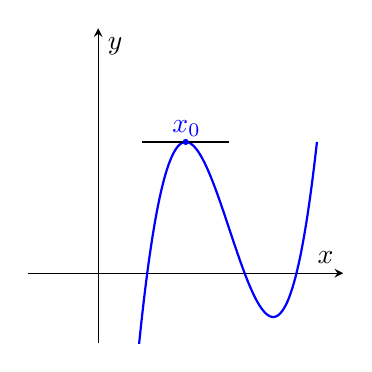
\begin{tikzpicture}
                \begin{axis}[
                xlabel=$x$,
                ylabel=$y$,
                axis equal,
                axis lines=middle,
                enlargelimits,
                xmax=5,
                xmin=-1,
                ymax=5,
                ymin=-1,
                xtick={0},
                ytick={0},
                scale only axis, 
                height=4cm, 
                width=4cm
                ]
            \addplot [blue, no marks, thick, domain=0:5, samples=1000] {(x-3)^3-3*x+10};
            \node at (2.02, 3.3) {\textcolor{blue}{$x_0$}};
            \addplot [thin] coordinates {(1, 3) (3,3)};
            \fill [blue] (2, 3) circle (0.07);
            \end{axis}
            \end{tikzpicture}
        \end{center}
        presenta in $ x_0 $ un punto di massimo locale; $ f $ è derivabile in $ x_0 $, e in questo punto la tangente è orizzontale.
        \item Per la funzione 
        \begin{center}
            \begin{tikzpicture}
                \begin{axis}[
                xlabel=$x$,
                ylabel=$y$,
                axis equal,
                axis lines=middle,
                enlargelimits,
                xmax=5,
                xmin=-1,
                ymax=5,
                ymin=-1,
                xtick={0},
                ytick={0},
                scale only axis, 
                height=4cm, 
                width=4cm
                ]
            \addplot [blue, no marks, thick, domain=0:5, samples=1000] {-sqrt(abs(x-1))+2};
            \node at (1.02, 2.3) {\textcolor{blue}{$x_0$}};
            \addplot [thin] coordinates {(0, 2) (2,2)};
            \fill [blue] (1, 2) circle (0.07);
            \end{axis}
            \end{tikzpicture}
        \end{center}
        $ x_0 $ è punto di massimo locale, ma la tangente in $ x_0 $ non è orizzontale perché non esiste.
    \end{enumerate}
}

\teorema[(di Fermat)]{difermatalleluia}{Se
    \begin{enumerate}
        \item $ f:I\to \R $, $ I $ intervallo;
        \item $ x_0 \in \mathring{I} $;
        \item $ x_0 $ punto di massimo o minimo locale;
        \item $ f $ derivabile in $ x_0 $;
    \end{enumerate}
    allora $ f'(x_0)=0 $, ovvero $ f $ ammette in $ x_0 $ tangente orizzontale.
}
\definizione{}{
    $ x_0 $ tale che $ f$ è derivabile in $ x_0 $ e $ f'(x_0)=0$ è detto \textit{punto critico} o \textit{stazionario} per $ f $.
}
\dimostrazione{difermatalleluia}{
    Studiamo il caso in cui $ x_0 $ punto di \textit{massimo} locale: \begin{equation}
        \exists\, U(x_0)\,\tc\quad \forall\,x \in U(x_0)\quad f(x)\le f(x_0)\: \bigl(\iff\, f(x)-f(x_0)\le 0\bigr)\label{eccociqui}
    \end{equation}
    Calcoliamo il limite: $\displaystyle
        \lim_{x\to x_0} \frac{f(x)-f(x_0)}{x-x_0}$: ci sono due casi.
    \begin{itemize}
        \item [(+)] Se $ x>x_0 $ \[
            \lim_{x\to x_0} \frac{f(x)-f(x_0)}{x-x_0} \underset{\footnotemark}{=}f'(x_0)\footnotetext{poiché $ f $ è derivabile in $ x_0 $}
        \]
        Vale inoltre $ f'(x_0)\le 0 $, per il teorema di permanenza del segno: infatti, nota \eqref{eccociqui}, si ha $ x-x_0>0 $.
        \item [(-)] Se $ x<x_0 $ \[
            \lim_{x\to x_0} \frac{f(x)-f(x_0)}{x-x_0} =f'(x_0)
        \]
        Inoltre $ f'(x_0)\ge 0 $ per il teorema di permanenza del segno: infatti, nota \eqref{eccociqui}, si ha $ x-x_0<0 $.
    \end{itemize}
    Allora deve essere \[
        f'(x_0)\le 0\:\land\: f'(x_0)\ge 0 \,\implies\, f'(x_0)=0
    \] %DOMANDA non mi piace questa dimostrazione, usare anche quella della piovano
}

\attenzione{
    Non vale il viceversa: un punto stazionario non implica un massimo (o un minimo).
}
\esempio{}{
    Sia $ f(x)=x^{3} $, $ \dom f=\R $: $ \forall\, x $, $ x \in \mathring{\R}$

    $ f'(x)=3x^{2} $, e $ f'(x)=0 $ $ \iff $ $ x=0 $, ma $ x_0=0 $ non è punto di massimo o minimo locale per $ f $. 

    $ x_0=0 $ è un flesso a tangente orizzontale\footnote{\hyperref[flesso]{definizione successiva}}.
}

\attenzione{Se $ x_0 $ è stazionario per $ f $, non è detto che sia massimo, minimo, o flesso a tangente orizzontale.}
\esempio{}{\label{esempiosinxquadrp}
    Data $ f(x)=\begin{cases}
        x^{2}\,\sin \frac{1}{x} & x\neq 0\\
        0 & x=0
    \end{cases} $ abbiamo verificato che $ f $ è derivabile in $ x_0=0 $, e $ f'(0)=0 $. $ x_0=0 $ è stazionario per $ f $, ma $ x_0=0 $ non è massimo, minimo o flesso. 
}
\begin{figure}
    \centering
        \begin{tikzpicture}
            \begin{axis}[
                xlabel=$x$,
                ylabel=$y$,
                axis equal,
                axis lines=middle,
                enlargelimits,
                xmax=0.05,
                xmin=-0.05,
                ymax=0.1,
                ymin=-0.1,
                xtick={0},
                ytick={0},
                scale only axis, 
                height=6cm, 
                width=6cm
                ]
            \addplot [blue, no marks, thick] file {xsin1x.csv};
            \end{axis}
        \end{tikzpicture}
    \caption{\hyperref[esempiosinxquadrp]{Esempio (\thesection.\theesempi)}}
    \label{figes:33}
\end{figure}

%TODO mancano tutte le cose successive, non si capiva assolutamente niente
% appunti di Simone Pacini